% !TeX root = skripta-konstitutivni-vztahy-materialu.tex
% !TeX lastmodified = 2019-04-01

\subsection{Model Neo-Hooke}\label{sec:neo-hooke}
\begin{itemize}
	\item NEO-HOOKE (1933-1934) 
	\item vědním oborem, který dal vznik tomuto modelu je „statistická mechanika“
	\item odvozen z představy o entropickém chování polymerních řetězců za předpokladu Gaussovského (normálního) rozdělení hustoty pravděpodobnosti poloh koncových bodů řetězců při jejich deformaci
	\item jedná se tak vlastně o první model, respektující strukturu materiálu (ať velmi elementárně, téměř nedokonale)
	\item Ve tvaru
\end{itemize}
\begin{equation}
	\psi = \frac{1}{2} G \left( \lambda_1^2 + \lambda_2^2 + \lambda_3^2 - 3 \right),
\end{equation}
přičemž
\begin{equation}
	G = N k T \sim \mu,
\end{equation}
kde
\begin{description}
	\item[$N$] je počet řetězců na jednotku objemu (počet částic daného množství)
	\item[$k$] je Boltzmanova konstanta $\SI{1.38064852e-23}{\joule\per\kelvin}$
	\item[$T$] he termodynamická teplota (zkrátka teplota)
	\item[$\mu$] je modul pružnosti ve smyku (u~nás značen $G = \frac{E}{2(1+\mu)}$, kde $\mu$ je Poissonovo číslo)
\end{description}

Také platí stavová rovnice ideálního plynu:
\begin{equation}
	p V = n R T = N k T \sim \mu
\end{equation}

Boltzmannova konstanta vyjadřuje vztah mezi teplotou a energií plynu. Vyjadřuje množství energie potřebné k zahřátí jedné částice ideálního plynu o jeden kelvin. Boltzmannova konstanta také úzce souvisí s entropií, protože stejně jako u entropie jde o množství energie na určitou teplotu. Byla pojmenována po rakouském fyzikovi Ludwigu Boltzmannovi, který se významně podílel na rozvoji statistické fyziky, kde tato konstanta hraje klíčovou roli.

Termodynamická teplota (též absolutní teplota nebo zkráceně teplota) je fyzikální stavová veličina dobře definovatelná protermodynamické systémy ve stavu termodynamické rovnováhy, rostoucí s růstem vnitřní energie systému. Její nerovnost určuje směr samovolného (tedy bez konání práce) přestupu tepla od teplejšího systému k systému chladnějšímu, uvedou-li se do tepelného kontaktu.

\subsubsection{Odvození}
Pro objasnění tvorby tohoto modelu je výhodně uvést i základní kroky vedoucí k jeho finální podobě

Základní předpoklady:
\begin{itemize}
	\item síť obsahuje obecně N řetězců na jednotku objemu
	\item žádná změna objemu během deformace (izochorický děj, nestlačitelný mat.)
	\item entropie sítě je dána součtem entropií jednotlivých řetězců
	\item koncové body mezi jednotlivými řetězci se při deformaci hýbou tak, jako by byly zality do elastického kontinua (afinní deformace)
\end{itemize}

\begin{figure}[H]
	\centering
	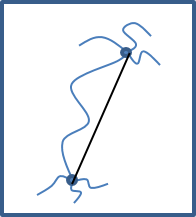
\includegraphics{Obrazky/sklon}
	\caption{Sklon pod úhlem $\alpha$}
	\label{fig:sklon}
\end{figure}
\begin{figure}[H]
	\centering
	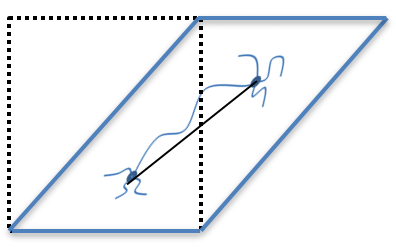
\includegraphics{Obrazky/sklon-rotace}
	\caption{Sklon pod úhlem $\alpha$ + rotace}
	\label{fig:sklon-rotace}
\end{figure}

Gaussovské rozdělení hustoty pravděpodobnosti poloh koncových bodů řetězce
\begin{figure}[H]
	\centering
	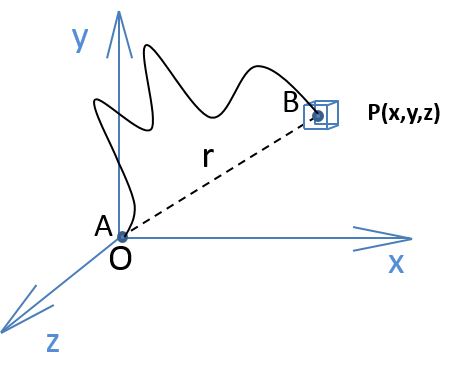
\includegraphics{Obrazky/kuhn}
	\caption{$P(x,y,z)$}
	\label{fig:kuhn}
\end{figure}
Kuhn (1934,1936) odvodil vztah, který reprezentuje pravděpodobnost, že složky vektoru $r$ definovaného spojnicí koncových bodů vlákna budou ležet v~intervalu:
\begin{equation}
od x do (x+dx)
od y do (y+dy)
od z do (z+dz)
\end{equation}
pravděpodobnost je
\begin{equation}
	p(x,y,z) \diff x \diff y \diff z
	= \frac{b^3}{\pi^{\frac{3}{2}}} \exp\left(-b^2(x^2 + y^2 + z^2)\right) \diff x \diff y \diff z
\end{equation}
přičemž
\begin{equation}
	b^2 = \frac{3}{2} n l^2
\end{equation}
a~uvažuje se $r << n l$
\begin{itemize}
	\item předpoklad, že vzdálenost není v~žádném případě srovnatelná s~nataženým řetězcem ($n l$)) 
	\item nezahrnuje také efekt postupného protažení (pak nutné použít ne-Gaussovské rozdělení)
\end{itemize}

Funkce je sféricky symetrická $x^2 + y^2 + z^2 = r^2$, proto
\begin{equation}
	p(x,y,z) \diff x \diff y \diff z
	= \frac{b^3}{\pi^{\frac{3}{2}}} \exp\left(-b^2(r^2)\right) \diff x \diff y \diff z
\end{equation}
pak zřejmě platí $p \rightarrow 1 \Leftrightarrow r \rightarrow 0$.

Distribuce spojnice koncových bodů vlákna -- distribuce $r$ vektoru (ne složek!!!)
\begin{figure}[H]
	\centering
	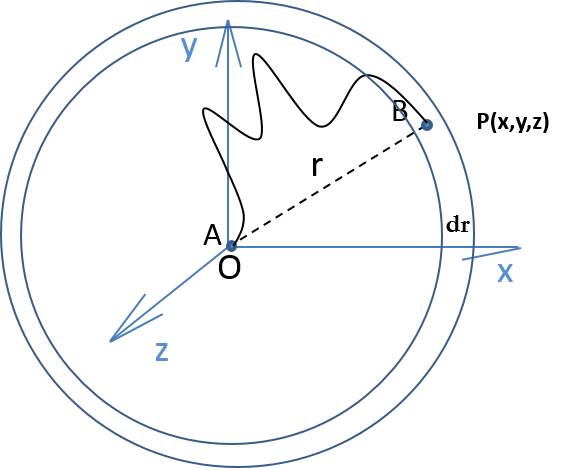
\includegraphics{Obrazky/distribuce-r}
	\caption{Distribuce $r$}
	\label{fig:distribuce-r}
\end{figure}

\begin{itemize}
	\item uvažujme všechny směry (x, y, z) stejně zastoupeny
	\item pak se bod B asi nepohybuje od x do x+dx, atd… ale je nutné aby se pohyboval např. po kulové skořepině s poloměrem r a elem. tloušťkou dr:
\end{itemize}
\begin{equation}
	P(r) \diff r
	= \frac{b^3}{\pi^{\frac{3}{2}}} \exp\left(-b^2(r^2)\right) 4 \pi r^2 \diff r
	= 4 \frac{b^3}{\pi^{\frac{1}{2}}} r^2 \exp\left(-b^2(r^2)\right) \diff r
\end{equation}
$P(r)$ je nulová při $r = 0$ a~dosahuje svého maxima ($r_m$) při: 
\begin{equation}
	\left(4 \frac{b^3}{\pi^{\frac{1}{2}}} r^2 \exp\left(-b^2 r^2\right)\right)
	= 0 \Rightarrow
	r_m = \frac{1}{b} = \sqrt{\frac{2 n l^2}{3}} \qquad\text{(příliš se však nepoužívá)}
\end{equation}
Důležitější je spíše hodnota střední hodnoty kvadrátu $r$, definovaná
\begin{equation}
	\bar{r^2} = \frac{\int_0^\infty r P(r) \diff r}{\int_0^\infty P(r) \diff r}
	= \frac{3}{2 b^2} = n l^2
\end{equation}

nyní se budeme snažit zjistit entropii jednoho řetězce a entropii soustavy řetězců (celé sítě). Začneme Boltzmanem (1887), který navrhl entropii (pro spojité izolované kontinuum) ve tvaru
\begin{equation}
	S = k \ln(\Omega),
\end{equation}
kde $\Omega$ charakterizuje část fázové prostoru (neboli počet rozlišitelných (mikro)stavů daného systému

Pravděpodobnostní prostor pohybu koncového bodu již máme definovaný
\begin{equation}
	\Omega = p(x,y,z) \diff \tau
	= \frac{b^3}{\pi^{\frac{3}{2}}} \exp\left(-b^2(r^2)\right) \diff \tau,
\end{equation}
tedy
\begin{equation}
	S
	= k \left\{\ln\left[p(x,y,z) \diff \tau\right]\right\}
	= k \left\{\ln\!\left(\frac{b^3}{\pi^{\frac{3}{2}}}\right) - b^2 r^2 + \ln(\diff \tau)\right\}
\end{equation}
z čehož vyplyne
\begin{equation}
	S = c - k b^2 r^2
\end{equation}

\begin{figure}[H]
	\centering
	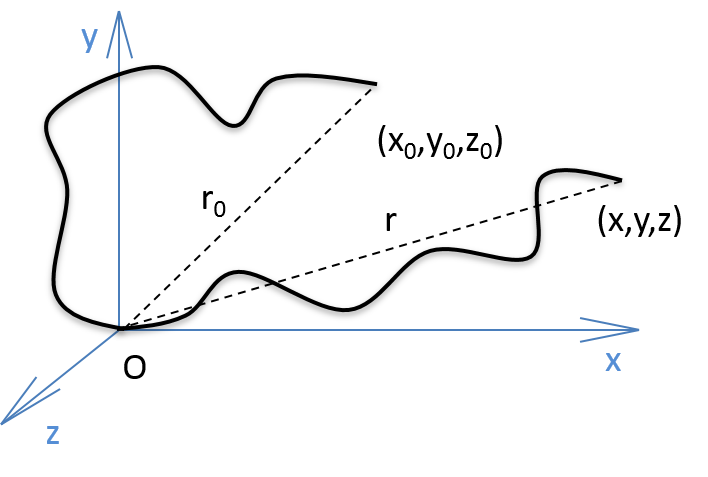
\includegraphics{Obrazky/neo-hooke-entropie}
	\caption{Řetězec}
	\label{fig:neo-hooke-entropie}
\end{figure}


\begin{itemize}
	\item entropie řetězce v~původním stavu:
	\begin{equation}
		S_0 = c - k b^2 r_0^2 = c - k b^2 (x_0^2 + y_0^2 + z_0^2)
	\end{equation}
	\item entropie řetězce v~deformovaném stavu
	\begin{equation}
		S = c - k b^2 r^2 = c - k b^2 (\lambda_1^2 x_0^2 + \lambda_2^2 y_0^2 + \lambda_3^2 z_0^2)
	\end{equation}
	\item příspěvek k~celkové entropii od tohoto jednoho řetězce
	\begin{equation}\begin{split}
		\Delta S &= S_0 - S
		= c - k b^2 (\lambda_1^2 x_0^2 + \lambda_2^2 y_0^2 + \lambda_3^2 z_0^2)
		- c + k b^2 (x_0^2 + y_0^2 + z_0^2)\\
		&= - k b^2 \left[ x_0^2(\lambda_1^2-1) + y_0^2(\lambda_2^2-1) + z_0^2(\lambda_3^2-1) \right]
	\end{split}\end{equation}
	\item Celková entropie sítě bude nejspíš součtem $N$ příspěvků $\Delta S$
	\begin{equation}
		S = \sum \Delta S = - k b^2 \left[ \sum x_0^2(\lambda_1^2-1) + \sum y_0^2(\lambda_2^2-1) + \sum z_0^2(\lambda_3^2-1) \right]
	\end{equation}
	$b$ je sice funkcí délky řetězce, nicméně pokud se předpokládá délka všech řetězců stejná, je $b$ konstantou
\end{itemize}

Protože jsou směry vektoru $r_o$ v~nezatíženém stavu zcela náhodné, nelze předpokládat žádnou preferenci směru $x$, $y$, nebo $z$. Tedy pravděpodobně platí
\begin{equation}
	\sum x_0^2 + \sum y_0^2 + \sum z_0^2 = \sum r_0^2
\end{equation}
a~zároveň
\begin{equation}
	\sum x_0^2 = \sum y_0^2 = \sum z_0^2 = \frac{1}{3} \sum r_0^2
\end{equation}
nicméně
\begin{equation}
	r_0^2 = N \bar{r_0^2},
\end{equation}
kde $\bar{r_0^2}$ je střední délka řetězců v~nedeformovaném stavu.

Po dosazení do celkové energie
\begin{equation}\begin{split}
	S &= \sum \Delta S
	= -\frac{1}{3} k N b^2 \bar{r_0^2} \left[ (\lambda_1^2-1) + (\lambda_2^2-1) + (\lambda_3^2-1) \right]\\
	&= -\frac{1}{3} k N b^2 \bar{r_0^2} \left( \lambda_1^2 + \lambda_2^2 + \lambda_3^2 - 3 \right)
\end{split}\end{equation}
kde
\begin{equation*}
	\bar{r_0^2} = \frac{3}{2} b^2
\end{equation*}
je entropie
\begin{equation}
	S = -\frac{1}{2} k N \left( \lambda_1^2 + \lambda_2^2 + \lambda_3^2 - 3 \right)
\end{equation}

Odvodili jsme entropii, ale potřebujeme energii \ldots otázkou tedy je, co dál?
Pomůže nám tzv. volná energie (Helmholtzova)
\begin{equation}
	\psi = U - TS
\end{equation}
Do které přispívají jak vnitřní energie (deformační energie přijata vychýlením se z~rovnovážných poloh daných vazbami krystalové mřížky), tak entropie (pocházející ze změny charakteru uspořádání). 

Ačkoliv se ani eleastomery nedeformuji čistě entropicky, příspěvek od vnitřní energie je často možné zanedbat proti příspěvku od změny entropie. 
\begin{equation}
	\psi = -TS = \frac{1}{2} k N T \left( \lambda_1^2 + \lambda_2^2 + \lambda_3^2 - 3 \right)
	= -\frac{1}{2} G \left( \lambda_1^2 + \lambda_2^2 + \lambda_3^2 - 3 \right)
\end{equation}

\subsubsection{Aplikace}
\begin{figure}[H]
	\centering
	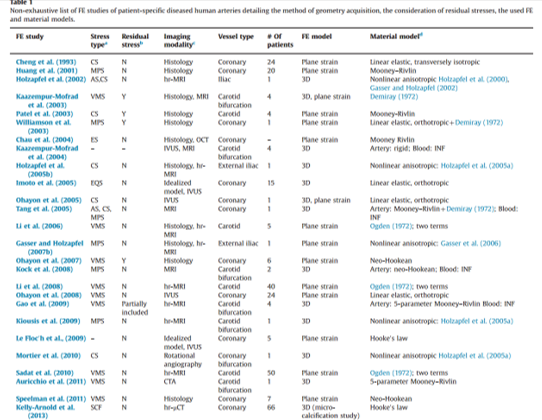
\includegraphics[width=0.7\linewidth]{Obrazky/neo-hooke-aplikace-1}
	\label{fig:neo-hooke-aplikace-1}
\end{figure}
\begin{figure}[H]
	\centering
	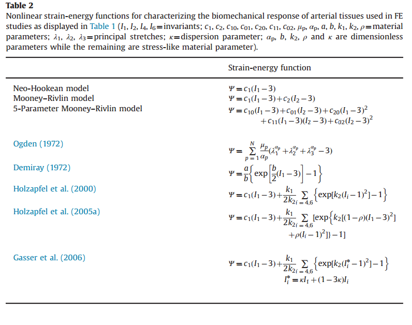
\includegraphics[width=0.7\linewidth]{Obrazky/neo-hooke-aplikace-2}
	\label{fig:neo-hooke-aplikace-2}
\end{figure}
\begin{figure}[H]
	\centering
	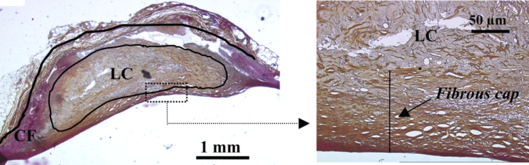
\includegraphics[width=0.7\linewidth]{Obrazky/neo-hooke-aplikace-3}
	\label{fig:neo-hooke-aplikace-3}
\end{figure}

\begin{align*}
	W = a (I_1 - 3)\\
	E_i \sim 6 a
\end{align*}

\begin{figure}[H]\centering\begin{tabular}{ll}\toprule
	Materiál & $E$\\ \midrule
	fibrosis & $\SI{500}{\kilo\pascal}$\\
	core & $\SI{5}{\kilo\pascal}$\\
	artery & $\SI{150}{\kilo\pascal}$\\
\bottomrule\end{tabular}\caption{Ohayon (2007)}\end{figure}

\subsubsection{Nenormální (neGaußovské) rozdělení pravděpodobnosti}
\begin{itemize}
	\item model Neo-Hook selhává při vyšších přetvořeních -- predikuje lineární odezvu, ač realita je silně nelineární
	\item důvodem je Gaussovské rozdělení pravděpodobnosti poloh koncových bodů vláken
	\item řešením je tedy použít ne-gaussovské rozdělení z čehož vznikají modely, jež bývají souhrnně označovány jako modely s~omezenou (někdy též limitovanou nebo konečnou) protažitelností řetězce -- limiting chain extensibility
	\item jedním z~nejznámějších je model \hyperref[sec:arruda-boyce]{Arruda-Boyce} (1998) nebo model Gent
\end{itemize}
